\chapter{Data sources and issues} \label{chap2}

\section{Student-level NAPLAN datasets used in the report}

Now I'm going to replace this line with something else...

The analysis in \textit{Closing the gaps} is based on linked student-level NAPLAN records.\footnote{Analysis was carried out for reading and numeracy, but not the other domains.} There are two major data sets used in the analysis:
\begin{itemize}
\item NAPLAN results across all four domains and year levels for all Australian students recorded in 2014, linked with their 2012 results where applicable.\footcite{acara2014} This dataset contains test scores for more than one million students for each domain in 2014, and more than 700,000 in 2012.\footnote{Only students in Years 5, 7, and 9 in 2014 have a linked record in 2012. Linked records are not available for students in the Northern Territory.}
\item NAPLAN results across all four domains recorded across 2009 to 2015 for the cohort of Victorian students who began Year 3 in 2009.\footcite{vcaa2015} For each domain, more than 55,000 students have a Year 3 test score and a score from at least one other test year. More than 45,000 students have a test score recorded in all of Years 3, 5, 7, and 9 for both reading and numeracy. 
\end{itemize}

Comparative year levels are estimated using the national data set to create a national benchmark for student progress. This benchmark is used in analysis of the linked Victorian data, which allows progress of individual students to be tracked from Year 3 to Year 9. In this way, the ``years of progress'' made by particular groups of Victorian students is relative to the typical Australian student, as opposed to the typical Victorian student.\footnote{This allows the analysis to pick up Victorian-specific effects. It should be noted that, on average, Victorian students score higher than most other states. One explanation for this is that Victorian students are, on average, about four months older than their counterparts from other states in the same year level, and are more likely to come from a high SES background [Grattan analysis of \textcite{acara2014}].}

The data contain a number of student background variables, including gender, parental education and occupation, language background and indigenous status. Some geographic information is available at the school level, including state, and whether the school is located in a metropolitan, regional, or rural area. The Victorian data also include the local government area of the school as well as a measure of school socioeconomic Status (SES): the Index of Community Socio-Educational Advantage (ICSEA).\footnote{To prevent school identification, this index is grouped into bands of 26 points.} The national data set contains a randomised school-level indicator -- it is possible to identify whether two or more students attend the same school, but not possible to identify schools themselves. 

Two additional data sets are used to check the robustness of the analysis across different cohorts -- the NAPLAN results across all domains and year levels for all Australian students recorded in 2013, linked with their 2011 results, and the NAPLAN results across all domains recorded across 2008 to 2014 for the cohort of Victorian students who began Year 3 in 2008.\footcite{acara2013,vcaa2014} Because NAPLAN results vary across cohorts, the analysis was rerun with these data. This confirmed that the key findings of the report -- in terms of the scale and direction of learning gaps -- were not cohort-specific.

\section{Defining the `typical' student}

The analysis presented in \textit{Closing the gaps} focuses on the `typical' student, either at the population level or within a particular sub-group of students. As noted in the main report and in \Cref{chap1}, for the purposes of measuring \textit{Years of Progress}, the typical student in a given year level is defined as the student with the median NAPLAN scale score. Analysis of particular sub-groups of students (such as those grouped by parental education or school SES) is performed according to the typical student within each sub-group -- the sub-group median.

An important advantage of using the median over the mean is that it is not directly affected by outliers. For instance, there may be a number of students who do not care about NAPLAN results who leave questions unanswered on the test instead of attempting them, meaning that their NAPLAN scale scores would not be an accurate estimate of their true ability. These inaccurate results would have a much larger impact on estimates of the mean score and the mean gain score than they would have on the median.\footnote{Estimates of the median would only be impacted in this way if a substantial number of students whose true ability is above the median are recorded below the median as a result of leaving questions unanswered.} NAPLAN scale scores also tend to have a small positive skew (particularly for numeracy), which lifts the mean relative to the median.

\section{Defining household socioeconomic status}

The report analyses how NAPLAN results and progress vary by socioeconomic status (SES), using the Victorian 2009--15 dataset. Variables relating to SES in the data include parental education, parental occupation, indigenous status and geographic location. One option would be to construct an index of household SES based on these variables. But there are issues constructing such an index for Victorian households. Firstly, very few students are indigenous and geographic location is only defined at the school level. Secondly, parental education and occupation are highly correlated -- for instance, 85 per cent of households where a parent has a Bachelor's degree are classified as a manager or professional, compared to only 21 per cent where no parent has a degree or diploma.\footnote{Grattan analysis of \textcite{vcaa2015}. Some studies use a composite measure of parental education and occupation, such as \textcite{marks2015,houng2015}, but a single measure is likely to still provide a reasonable proxy for household SES.}

We instead use a simple proxy for household SES: the highest level of parental education attained. While there is information on the highest schooling year attained, most parents of school-age children in Victoria have completed Year 12; we therefore focus on educational attainment beyond school.\footnote{Studies have shown that post-school qualifications are a strong predictor of household income; see, for instance \textcite{oecd2015}.} Students can be divided into four groups based on the highest level of parental education:
\begin{itemize}
\item at or above Bachelor's degree
\item diploma
\item certificate I to IV
\item year 12 or below.
\end{itemize}

\Cref{fig:parental_ed} shows that each of these four categories include at least 15 per cent of all students. Preliminary analysis suggests that the difference in student attainment and progress between the lowest two categories of parental education is small -- the report groups these into a single category: `below diploma'.

\begin{figure}[t]
 \captionwithunits{Students are well represented in each category of parental education}{Percentage of students, Victoria 2009--15 cohort}
 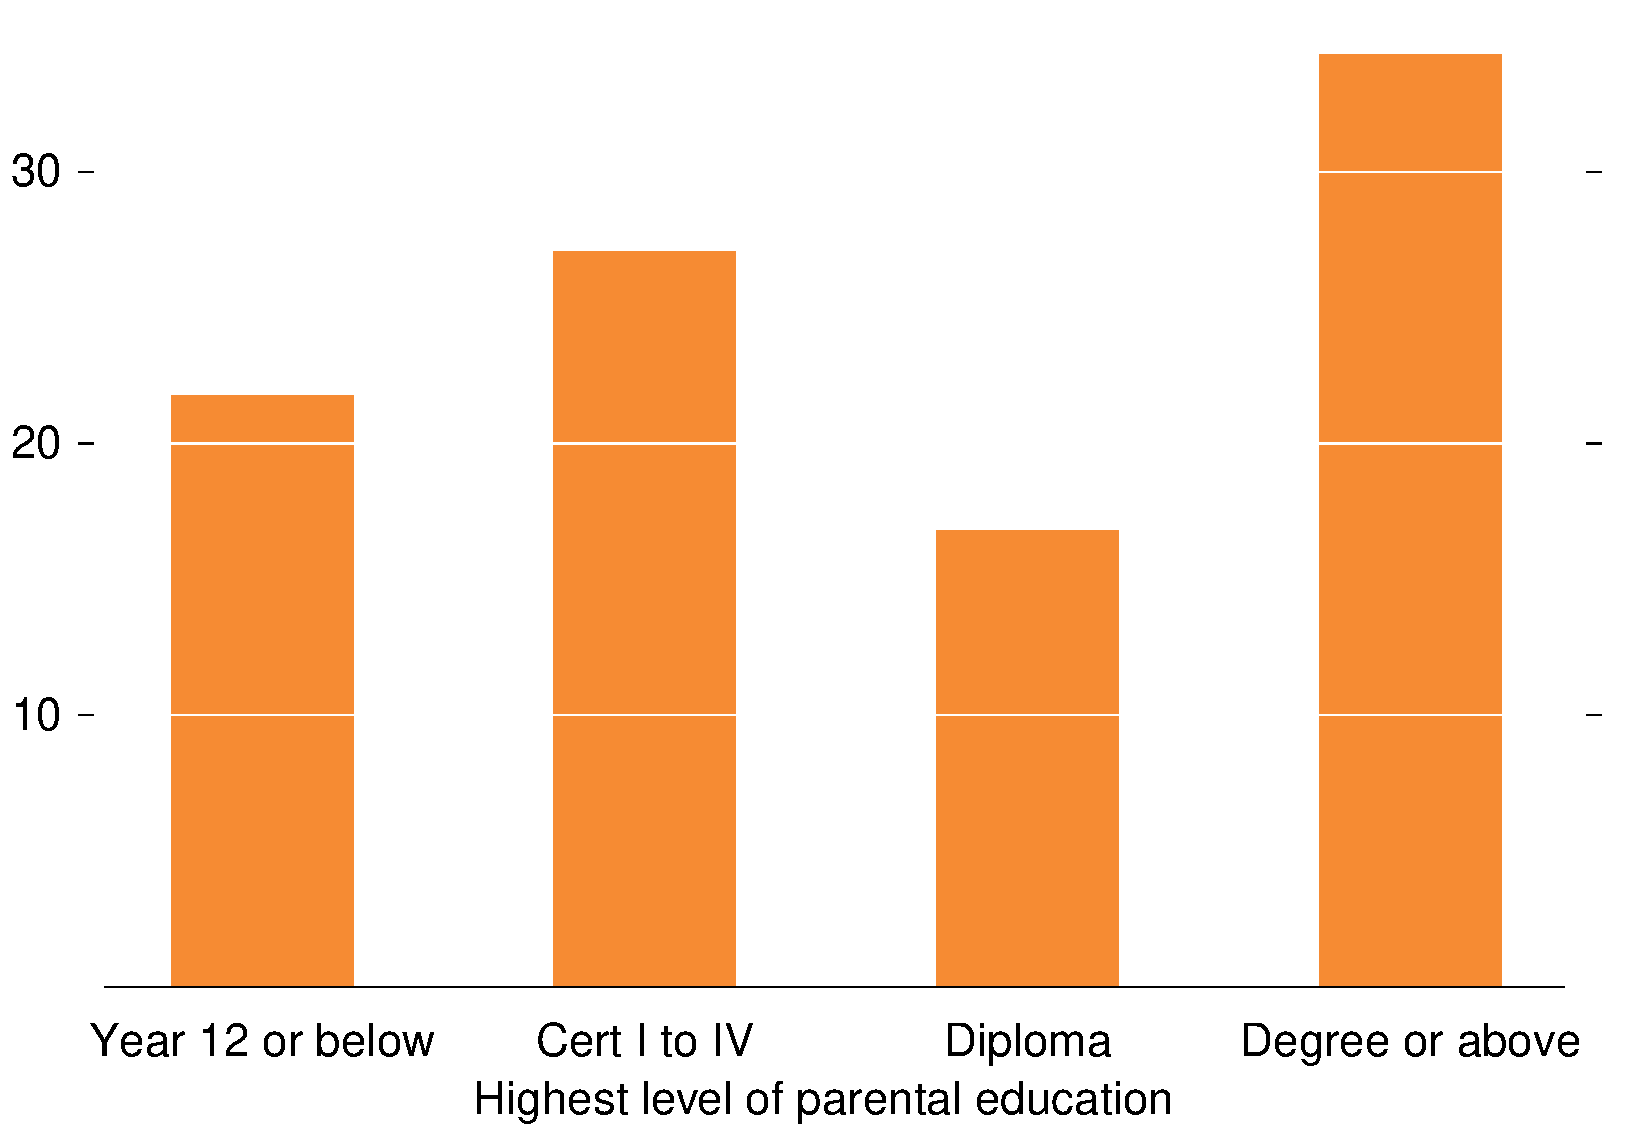
\includegraphics[width=\columnwidth]{atlas/Parental_ed.pdf}\label{fig:parental_ed}

\source{Grattan analysis of \textcite{vcaa2015}.}
\end{figure}

\section{Using ICSEA as a measure of school socioeconomic status} \label{sec:icsea}

The report analyses how NAPLAN results and progress vary by the Index of Community Socio-Educational Advantage (ICSEA, which is referred to in the report as `school SES') in the Victorian 2009--15 dataset. ICSEA was developed by ACARA so that NAPLAN results could be compared between schools with similar student backgrounds. The index is based on student-level factors such as parental education and employment, indigenous status, and school-level factors such as remoteness and the proportion of indigenous students.\footnote{Geographic census data are also used in the index calculation.} The index is constructed as a linear combination of these SES variables.

To determine the weighting applied to each variable, a regression model is estimated: average NAPLAN score (across all domains) against each SES variable. The estimated parameters of this model determine the weightings -- essentially this means that the SES variables are weighted according to how strongly they relate to NAPLAN results. This index is then averaged across all students in each school, and scaled nationally so that the ICSEA distribution has a mean of 1000 and a standard deviation of 100. This methodology provides an estimate of ICSEA for each school, which is adjusted each year.\footnote{For more detail, see \textcite{acara2014a}.}

In each schooling year, school ICSEA is allocated to one of three groups:
\begin{itemize}
\item ICSEA greater than 1090 (approximately the top quartile of schools in Victoria)
\item ICSEA greater than 970 but less than 1090 (approximately the middle two quartiles of schools in Victoria) 
\item ICSEA less than 970 (approximately the bottom quartile of schools in Victoria).\footnote{This cut points were chosen from the ICSEA bands available to us. It should be noted that the average ICSEA of Victorian schools is higher than the national average.}
\end{itemize}

There is a question as to whether the strong relationship observed between school SES and NAPLAN results is legitimate, or whether it arises as a result of the way ICSEA is constructed. While NAPLAN results are used in the construction of ICSEA, they are not used as an input variable -- ICSEA is still entirely a linear function of SES variables. This means that the strong relationship observed between ICSEA and NAPLAN results is driven by SES factors, not by the way the index is constructed.

\section{Missing data} \label{sec:missing}

There are two major sources of missing NAPLAN data: non-participation in NAPLAN and results that are not linked for the same student in different years. The non-linkage of results is only an issue for students in the Northern Territory -- no linked data are available for Northern Territory in the national dataset.

For any given NAPLAN test, participation rates are high, usually exceeding 90 per cent. The most common reason for non-participation is student absenteeism. This is usually four per cent or less, but rises to seven per cent in Year 9, as shown for numeracy in \Cref{fig:absent_pc}. A small proportion of students (typically less than two per cent) are given an exemption from taking the NAPLAN test, usually if they have a significant disability or face a major language barrier. Finally, some students are withdrawn from testing by their parent/carer, although this is less than two per cent on almost every test.

\begin{figure}[t]
 \captionwithunits{Students are more likely to be absent from a NAPLAN test in Year 9}{Percentage of students that are absent from NAPLAN numeracy test, Victorian 2009-2015 cohort}
 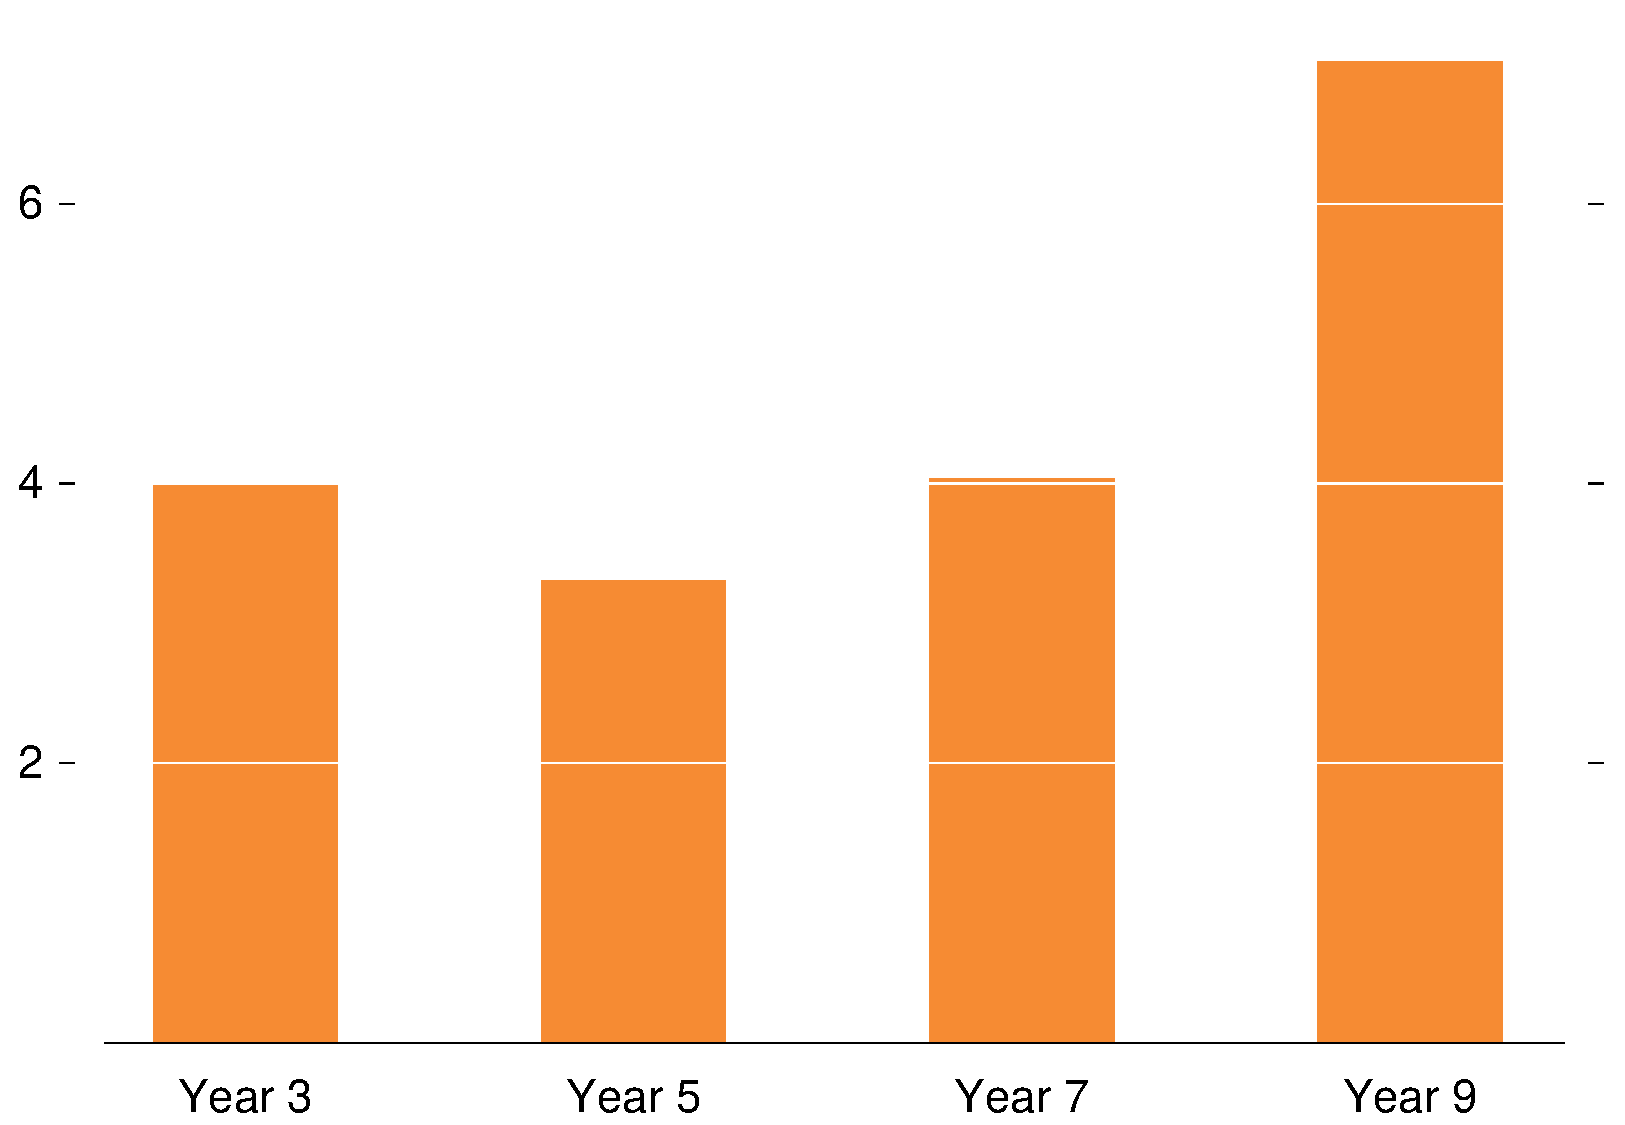
\includegraphics[width=\columnwidth]{atlas/Absent_pc.pdf}\label{fig:absent_pc}
\notes{Does not include students who are exempt, withdrawn or miss a test due to leaving Victoria. Results are similar for reading.}

\source{Grattan analysis of \textcite{vcaa2015}.}
\end{figure}

Despite a high participation rate on each test, these missing data can potentially reduce the size of the linked samples quite significantly. In the cohort of Victorian students who took the Year 3 test in 2009, only about 72 per cent took all four NAPLAN tests to Year 9 for numeracy and reading. This is because different students missed the test in different years, and also because some students moved out of Victoria before Year 9.\footnote{There are also students that accelerate or repeat a year -- these students are included in the analysis, although some have not completed Year 9 by 2015.}

\begin{figure}[t]
 \captionwithunits{Students from lower SES backgrounds are more likely to miss one or more NAPLAN tests}{Percentage of students that miss a NAPLAN test, Victoria 2009--15 cohort}
 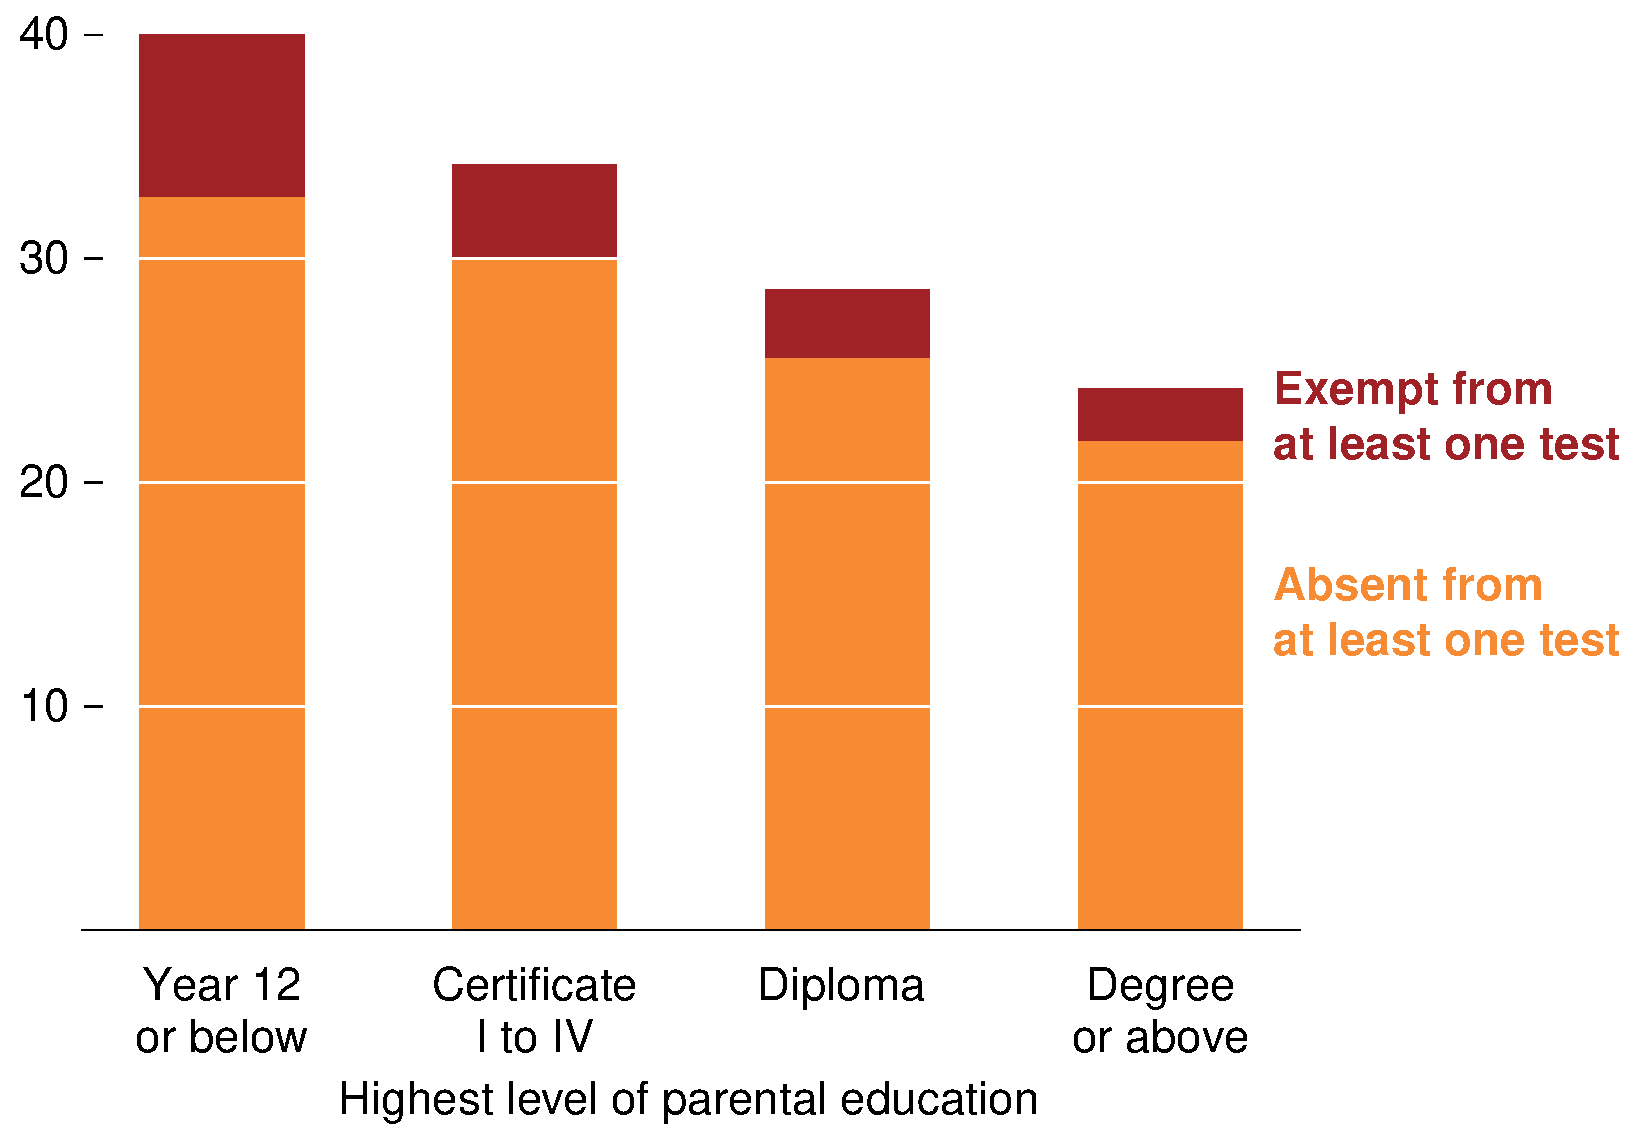
\includegraphics[width=\columnwidth]{atlas/Missing_SES.pdf}\label{fig:missing}
\notes{Includes all Victorian students in Year 3 in 2009, and all NAPLAN tests taken up to 2015. `Absent from at least one test' includes those who were withdrawn, and those not in Victoria in one or more test-taking years after Year 3. Students that have been both absent and exempt from tests are categorised as exempt.}

\source{Grattan analysis of \textcite{vcaa2015}.}
\end{figure}

A brief analysis suggests that students are more likely to miss a test due to being absent/withdrawn or an exemption if they are from a low SES background. \Cref{fig:missing} shows that of the Victorian cohort of students in Year 3 in 2009, 40 per cent of those whose parents have no tertiary education missed at least one test between Year 3 and Year 9, compared to only 25 per cent of students where a parent has a Bachelor's degree.

Given that students from high SES backgrounds typically score higher and make higher gains from a given starting score than those from low SES backgrounds, the consequence of ignoring missing data is an upwards bias in estimates of the median score and median gain score.\footnote{That is, the estimated median is likely to be above the actual population 50th percentile.}

\begin{figure}[t]
 \captionwithunits{Missing data have more of an impact on gain scores for students from low SES backgrounds}{Median NAPLAN gain score by highest level of parental education, reading, Year 5 to Year 7}
 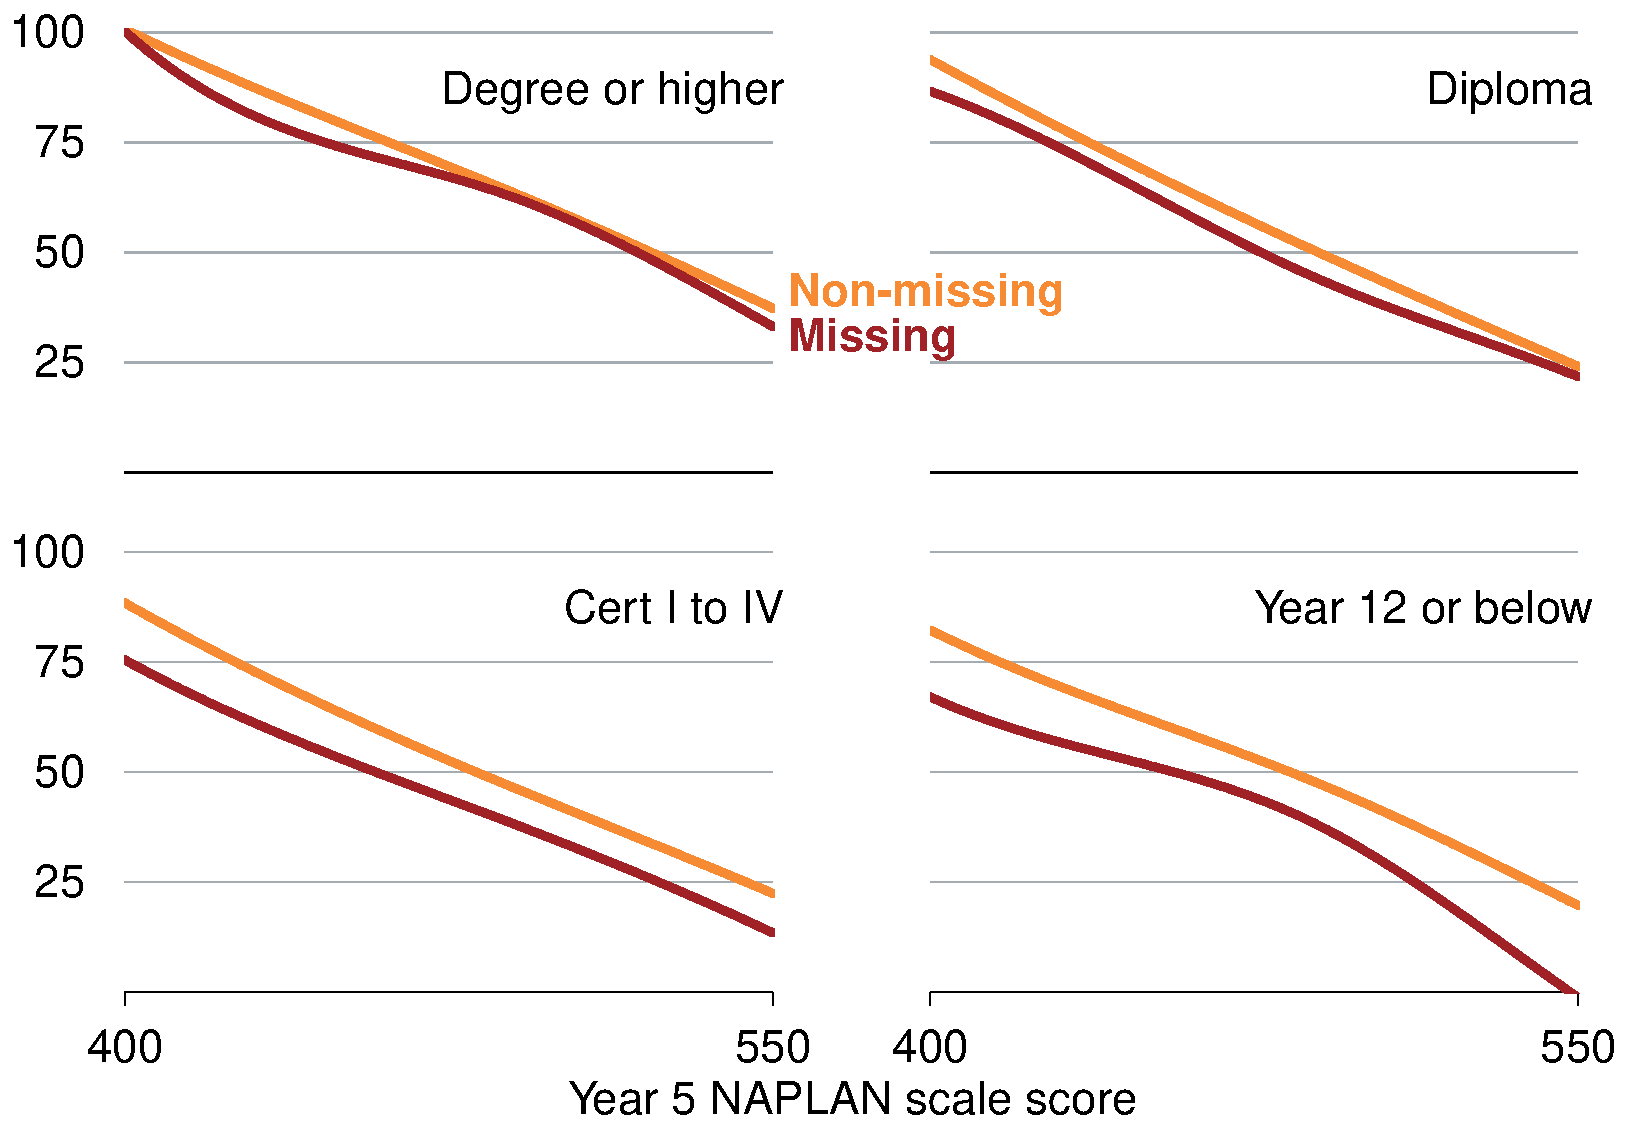
\includegraphics[width=\columnwidth]{atlas/Missing_gain.pdf}\label{fig:missing_gain}
\notes{`Missing' includes all students that were absent/withdrawn from either the Year 3 or Year 9 reading test, but does not include exempt students. `Non-missing' includes all students that did not miss a single NAPLAN test. A similar pattern exists for numeracy, for other year levels, and for school-level SES.}

\source{Grattan analysis of \textcite{vcaa2015}.}
\end{figure}

For analysis that tracks the progress of a particular sub-group, such as students that have a parent with a Bachelor's degree, missing data may be associated with lower gain scores from a given starting score. With only two years of linked data it would not be possible to test this. But with four years of linked data, as is available with the Victorian 2009 to 2015 cohort, there are students that have missed a test in one or two years, but for whom we observe NAPLAN scale scores in at least two other years. \Cref{fig:missing_gain} shows the estimated median gain score in reading between Year 5 and Year 7 for students that did not miss a test in any year, and for students that missed a test in Year 3, Year 9 or both. Not only are those that missed a test predicted to make smaller gains, but the gap is larger for students from low SES backgrounds (using parental education as a proxy).

This means that estimates of median progress for particular sub-groups are likely to be upwards biased if missing data are ignored. But the bias is likely to be much larger for low SES groups. In turn, this means the gaps in student progress between high and low SES students are likely to be underestimated rather than overestimated.\footnote{The report shows a very consistent pattern of high SES students out-performing low SES students in Year 3, and this gap growing over time. This is a key finding of the report. Missing data would be more problematic if the consequence was overestimating these gaps.}

Our analysis of NAPLAN gain scores does not impute missing results. Students who are given an exemption from one or more tests are excluded from the analysis.\footnote{For the purposes of reporting, ACARA assume exempt students are performing below the national minimum standard. Imputing NAPLAN scale scores for these students would change the sample median, but with so few students exempt it is unlikely the results would change significantly.} When estimating progress for Victorian students, we take an approach that aims to minimise bias -- rather than excluding all students that miss a test, we include all students that undertook the Year 3 test and at least one other test. This approach is outlined in more detail in Section \ref{sec:ses_sub}.

\newpage
\section{Measurement error and bias}

\subsection{Measurement error at the student level}

The NAPLAN scale score that a student receives for a particular test is known as a `weighted likelihood estimate' (WLE).\footnote{These are also referred to as `Warm's Estimates'; see \textcite{warm1989}.} Two students that answer the same number of correct answers on the same test receive the same WLE.

The score that a student receives on the NAPLAN test provides an estimate of their true current ability in a particular domain, but this is subject to substantial measurement error. The accuracy of the estimate increases with the number of questions asked.\footnote{On the Year 3 numeracy test in 2009, for instance, there are 35 questions, and NAPLAN scale scores are estimated with a standard error between 24 and 35 for the vast majority of students. On the Year 9 numeracy test in 2015, there are 64 questions, and the standard error of NAPLAN scale scores is between 17 and 30 for nearly all students. Extreme scores (nearly all questions correct/incorrect) are estimated with much higher standard errors [\textcite{acara2015d}].} Two scores are needed to estimate progress over time, and each is subject to measurement error. It is therefore difficult to accurately estimate the progress of an individual student using NAPLAN results.

NAPLAN results are more accurate for estimating the progress of a sizeable group of students, as measurement error is reduced when results are aggregated across students. But simply aggregating does not solve all of the potential measurement error issues. This section outlines these issues in detail and explains the approach we have taken to mitigate them.\footnote{There may also be measurement error issues in other variables -- for instance, parental education may change over the course of a child's schooling years, but this is not recorded. Our analysis assumes that the recording of background variables is accurate.}

\subsection{Using NAPLAN scale scores (WLEs) may result in imprecise estimates of progress}

\subsubsection*{Ability is continuous, but NAPLAN scale scores are discrete}

NAPLAN scale scores provide an estimate of student ability, a continuous latent variable. But because there are a finite number of questions on each NAPLAN test, the estimates of student ability (NAPLAN scale scores) have a discrete distribution. This can add greater imprecision in estimating percentiles (including the median) and gain scores.

On the Year 3 numeracy test, for example, there are only 35 questions, meaning that there are only 35 possible NAPLAN scale scores a student can receive. The cohort of students that takes the test in 2014 would receive a different set of scores to the cohort taking the test in 2015, even where there is no significant difference between the two cohorts.\footnote{A histogram comparing two cohorts would show a similar overall distribution, but the estimated points on the NAPLAN scale would be different.} Ignoring the discrete nature of the estimates could overstate the difference between two cohorts because of `edge effects', especially when comparing performance in terms of percentiles, such as the progress or achievement of the median student.

This is best dealt with in two ways. First, adjust for the discrete nature of NAPLAN scale scores (as described in \Cref{sec:pv}). Second, take care when comparing cohorts across years.\footnote{In particular, if a particular cohort is used to generate a progress baseline to assess achievement or progress of students from a different cohort, this would increase measurement error.}

\subsubsection*{Regression to the mean}

In the context of comparing student progress over two or more NAPLAN tests, \textit{regression to the mean} suggests that an extreme NAPLAN score in one year (either extremely low or high) is likely to be followed by a less extreme score on the following test (two years later). This is not because students at the extremes are making significantly high/low progress, but because the original test score is exaggerated by measurement error. This may lead to learning progress being significantly overstated by gain scores for students who start with a very low score, and understated for students who start with a very high score.\footnote{The data show a systematic pattern of high gain scores for low prior scores and low gain scores for high prior scores; see, for example, \Vref{fig:gain_prior} and \Vref{fig:missing_gain}. But if this were entirely due to regression to the mean, we would expect the path of progress for the median student from Year 3 to Year 9 to be approximately linear -- this is clearly not the case.}

\textcite{wu2005} notes that the average of the WLEs provides an unbiased estimate of the population mean ability, but the sample variance overstates the population variance. This bias disappears as the number of test questions increases. For students who score close to the mean, the bias in the WLE as an estimate of their ability will be small. But for extreme percentiles, the bias can be large.\footnote{A way to think about this is that the effective number of questions declines as student ability moves further from the level at which the test is set. For example, a student at the 90th percentile will find most questions too easy, while a student at the 10th percentile will find most questions too difficult. Only a few questions will be set at an appropriate level for such students. The move to NAPLAN online will allow better targeting of questions, reducing the measurement error at the extremes.}

It is important to note that an extreme score for a particular sub-group might not be an extreme score for another sub-group. For example, the NAPLAN scale score equal to the 95th percentile in Year 7 numeracy for those whose parents have no post-school qualifications is only at the 82nd percentile for those who have a parent with a Bachelor's degree. This means that the regression to the mean between the Year 7 and Year 9 test is likely to be stronger for a high achieving low SES student than it is for a high achieving high SES student.\footnote{This does not mean that all high NAPLAN scale scores for low SES students are overstating their true ability. But when we compare a low SES and a high SES student with the same high score, the low SES student is more likely to have had a particularly good test day than the high SES student.}

\subsection{Approaches to mitigate the impact of measurement error and bias} \label{sec:pv}

\subsubsection*{Simulation approach}

All WLEs (NAPLAN scale scores) are point estimates and are associated with a standard error. \textcite{warm1989} shows that these estimates are asymptotically normally distributed. Using this property, we approximate the distribution of student ability, $\theta$, given these estimates:
\begin{equation}
\theta_{n} \overset{a}\sim \mathcal{N}\left(\widehat{\mu}_{n},\widehat{\sigma}_{n}^{2} \right)
\end{equation}
where $n$ is the number of questions correctly answered, $\widehat{\mu}_{n}$ is the corresponding WLE, and $\widehat{\sigma}_{n}^{2}$ is the variance of the WLE. 

For each student, we simulate a NAPLAN scale score (an ability level) as a random draw from this distribution.\footnote{This is performed for each year in the Victorian cohort and each year in the national dataset, using the standard errors reported by \textcite{acara2015d}.} This creates a sample that has the properties of a continuous distribution, allowing for more accurate estimates of percentiles.

\begin{figure}[H]
 \captionwithunits{The simulation approach solves the issues of discrete NAPLAN scale scores}{Histogram of Year 5 NAPLAN scale score, numeracy}
 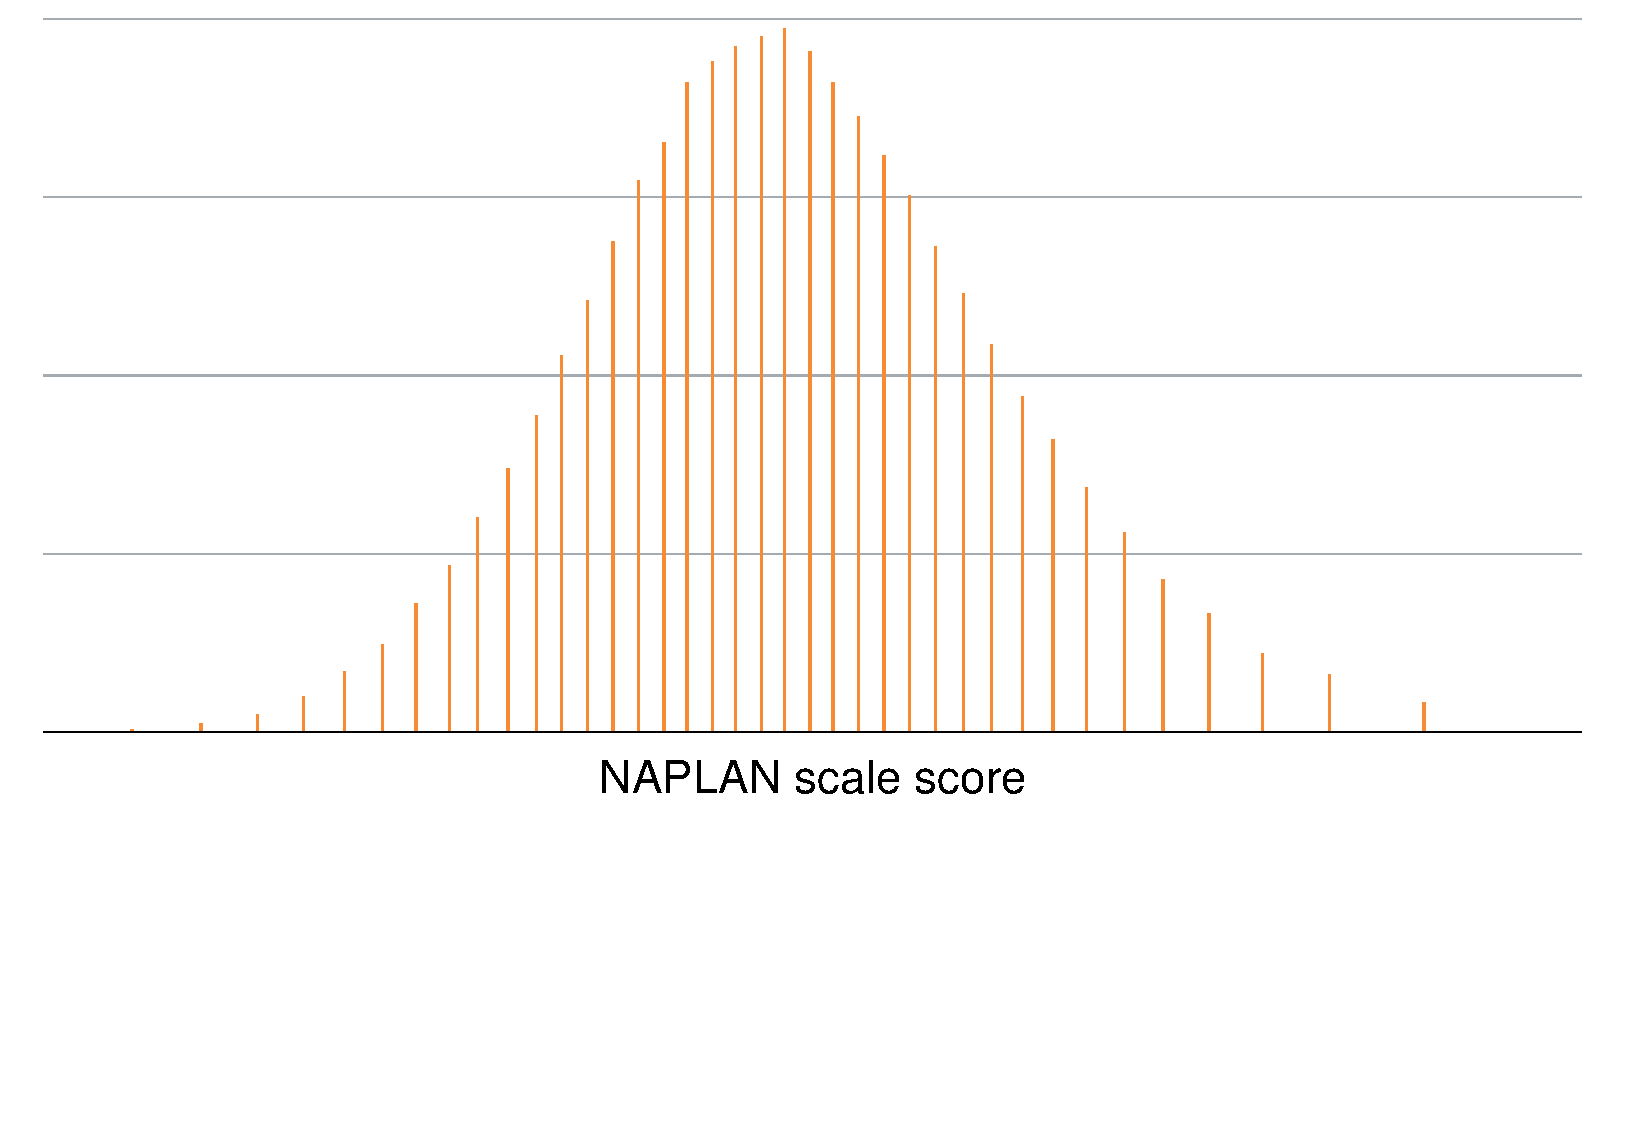
\includegraphics[width=\columnwidth]{atlas/Hist_NSS.pdf}\label{fig:histogram}
  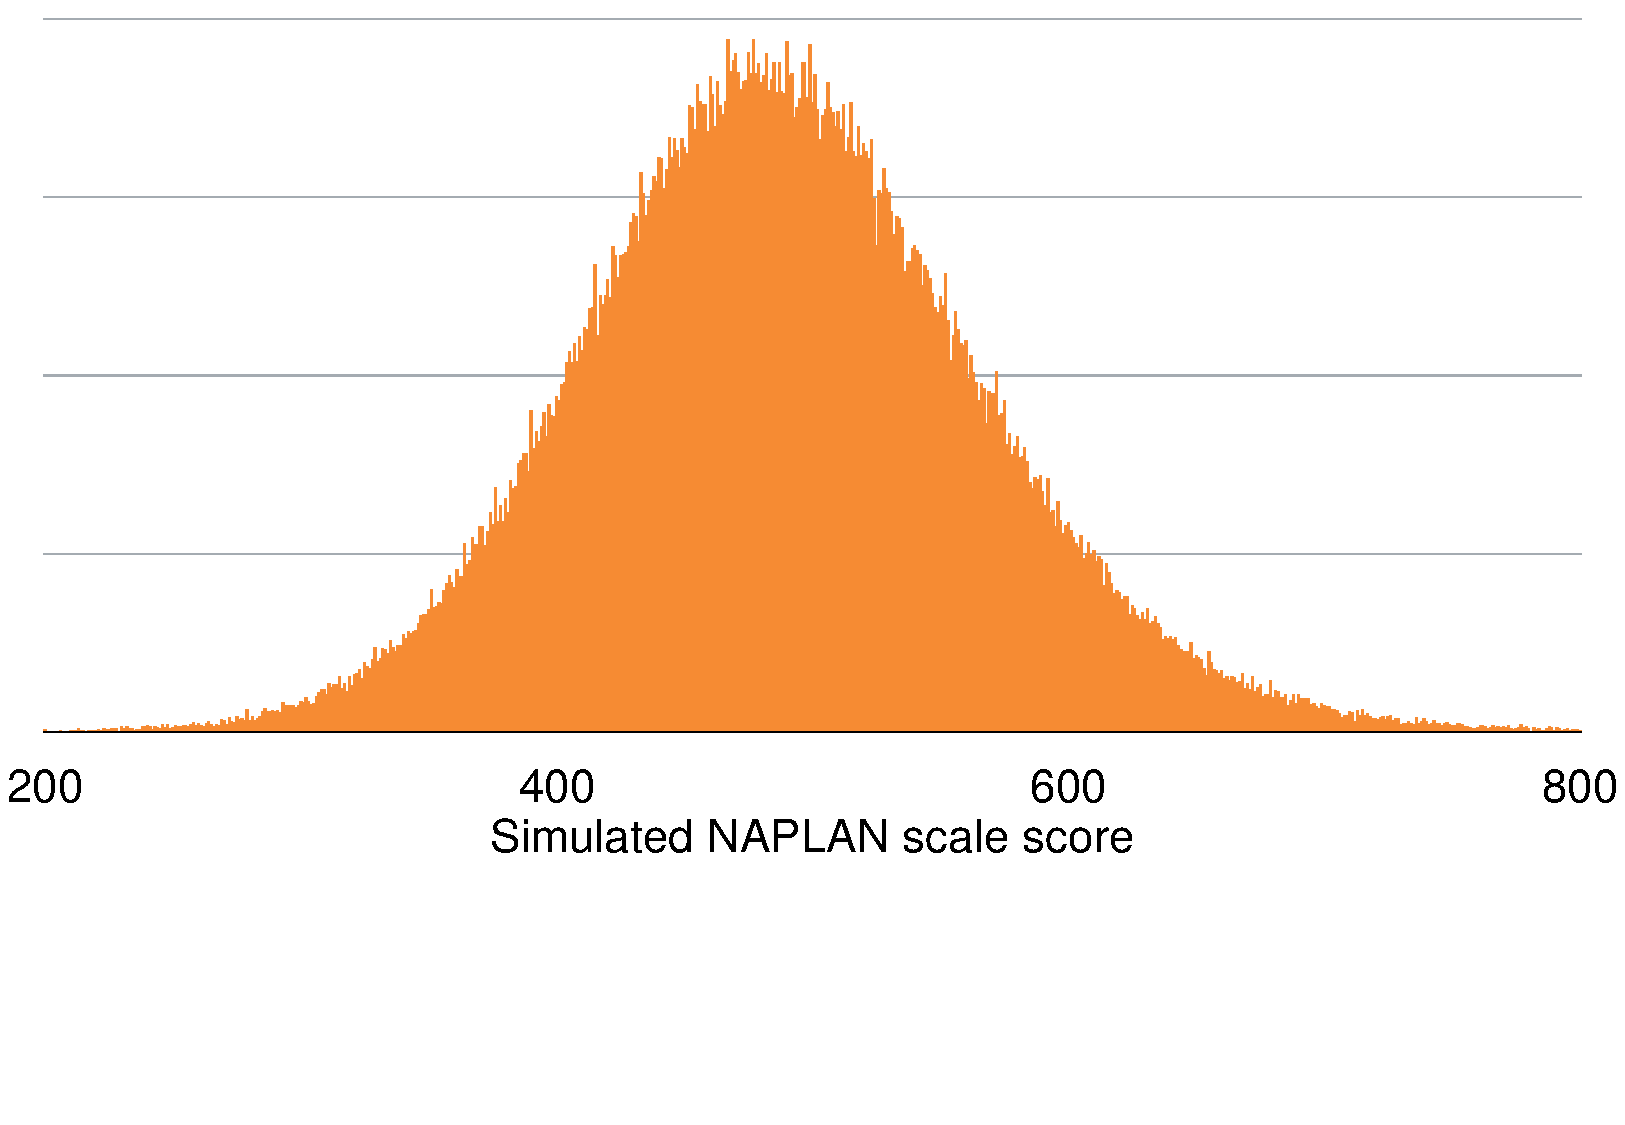
\includegraphics[width=\columnwidth]{atlas/Hist_SIM.pdf}
\notes{Frequency is not shown on Y-axes, but scaled so that both charts can be compared. Bin width = 0.5.}

\source{Grattan analysis of \textcite{acara2014}.}
\end{figure}
%\vspace{-6pt}
\newpage
While this approach does not remove measurement error at the individual student level, it takes into account that measurement error varies across students with different scores. \Cref{fig:histogram} compares a histogram of discrete NAPLAN scale scores to a histogram of simulated NAPLAN scale scores.

\subsubsection*{Use of sub-groups with large samples}

Simulating NAPLAN scale scores does not remove measurement error at the individual student level. In fact, it increases the standard error associated with an individual student estimate and gain score.\footnote{This approach would be inappropriate for reporting individual student results.} We keep this measurement error to a minimum by aggregating students into sub-groups that have large samples, and calculating our results based on five sets of random draws.\footnote{The standard error due to measurement in a sub-group is proportional to $\sqrt{n}$, the square root of the sub-group sample size. For a sub-group with 10,000 people, the standard error will be 100 times smaller than it will be for an individual student.}

\verb+insert table showing sample sizes for different sub-groups+

\subsubsection*{Avoiding extreme percentiles}

There is no straightforward way to estimate the magnitude of the bias in the WLEs for different percentiles. But it is well known that the magnitude of the bias due to regression to the mean is largest for extreme percentiles, and that the bias is small for percentiles close to the median. The impact of regression to the mean is also larger when the correlation between two measurements (such as test scores) is weak. In our sample, the correlation between NAPLAN test scores across two test-taking years for a given domain is between 0.75 and 0.8 -- this strong correlation suggests regression to the mean will have only a small impact for most percentiles.

Nonetheless, our analysis aims to avoid estimating NAPLAN scale scores and gain scores for students at extreme percentiles, and most analysis is focused around the median student. We use a rule of thumb to minimise bias due to regression to the mean -- no analysis is based on the estimated NAPLAN scale score or gain score of students below the 10th percentile or above the 90th percentile.\footnote{These extreme percentiles are avoided both for the overall population, and for particular sub-groups.}

In constructing the benchmark curve to estimate comparative year levels (outlined in \Vref{chap3}), it is necessary to estimate the median gain score of below-average students from Years 3 to 5, and above-average students from Years 7 to 9. It is possible to estimate the NAPLAN scale score for a student as low as six months below Year 2 level, and as high as Year 12 level without using extreme percentiles.

For the analysis of progress using Victorian data, we track low, medium, and high achieving students based on their percentile at Year 3 -- the 20th, 50th, and 80th at the population level. But these percentiles can be more extreme when analysing sub-groups. In numeracy, for example, the 20th percentile across the population is equal to the 12th percentile for students who have a parent with a Bachelor's degree, and the 80th percentile at the population level is the 87th percentile when the highest level of parental education is below a diploma. \Cref{tab:percentiles} shows the within-group percentiles for different levels of parental education -- none of these are more extreme than the 10th or 90th percentiles.

\begin{table}[htbp]
  \centering
  \captionwithunits{Analysis of particular sub-groups does not extend beyond the 10th or 90th percentiles within each group}{Within-group percentile in Year 3 numeracy by parental education}
    \begin{tabular}{lccc}

  & \multicolumn{3}{c}{Percentile} \\
\cmidrule(lr){2-4}
    \textit{Population} & \textit{20}    & \textit{50}    & \textit{80} \\
    Degree or above & 11.9  & 37.1  & 70.8 \\
    Diploma & 19.7  & 50.1  & 81.5 \\
    Below diploma & 26.3  & 59.5  & 86.7 \\
    \bottomrule
    \end{tabular}%
  \label{tab:percentiles}%
\begin{flushleft}\source{Grattan analysis of \textcite{vcaa2015}.}\end{flushleft}
\vspace{-6pt}
\end{table}%

\newpage
Nonetheless, the gaps in progress between high and low SES may still be overstated due to regression to the mean, particular when starting from either the 20th or the 80th percentile in Year 3. This is explore more in Section \ref{sec:robust_progress}.

\subsubsection*{Reporting of results and standard errors}

The report does not show standard errors or confidence bounds on point estimates of NAPLAN scale scores or comparative year levels. But confidence bounds are estimated to ensure the significance of reported results. We calculate 99 per cent confidence intervals using a bootstrap approach with 200 replications, each with a different set of random draws.

We estimate a confidence interval for the benchmark comparative year level curve, as well as confidence intervals for the analysis of progress using the Victorian cohort. For results that are reported in terms of comparative year levels or years of progress, these confidence intervals are conservatively estimated -- we use the upper and lower bounds estimated for the benchmark curve, combined with the upper and lower bounds on the point estimates of NAPLAN scale scores. This approach takes into account the measurement error in the Victorian cohort, as well as the measurement error in the estimation of comparative year levels.

The confidence bounds are used to validate our analysis for robustness -- we do not draw conclusions from any results that are not statistically significant (including gaps in progress between different groups). The report notes any case in which an estimated comparative year level has a standard error of three months or more. 

\verb+insert table/chart showing example of confidence interval+

Full results with confidence bounds are available for download (\verb+insert link+).

\subsubsection*{Plausible values}

The best approach that could be taken to reduce the impact of measurement error would be to use plausible values. Like the simulation approach outlined above, this approach would simulate a NAPLAN scale score from a continuous distribution for each student, including imputing values for missing data. But plausible values are simulated from a distribution that takes into account student and school background factors.\footnote{In theory these could also take into account NAPLAN scores in other year levels.} NAPLAN reports produced by ACARA are based on analysis using plausible values.\footcite[][22]{acara2015a}

When simulated correctly, plausible values are able to produce unbiased estimates of percentiles and gain scores for each sub-group.\footcite{wu2005} Plausible values were, unfortunately, only available for the 2014 test year in the national dataset, but not for the 2012 results or the Victorian 2009--15 cohort. This means we did not have the data to use plausible values to analyse progress.\footnote{In any case, the 2014 plausible values are, to the best of our knowledge, generated independently of prior test scores. Analysing student progress would require that plausible values are simulated from a distribution that takes prior test scores into account.}

We do, however, utilise the 2014 plausible values (generated by ACARA) for estimating the population distribution of results for each year level. These estimates therefore take missing data and measurement error into account. 